\section{Lookup Tables (LUTs)}
An interesting approach to build a network without backprop is described in \cite{chatterjee2018learning}. The input is a $d$-dimensional boolean vector and the output is either 0 or 1. The basic idea is to build a \enquote{lookup table} (LUT) based on the training data. Many lookup tables (LUTs) are created and stacked, reminding us of a neural network. The paper shows that this architecture not only generalizes on yet unseen data, but also shares some properties of neural networks. Let us first start with the definition of a single LUT and then work our way up to a network of LUTs. We then discuss experimental results of \cite{chatterjee2018learning} which we also re-create on our own.

\subsection{Single lookup tables (LUTs)}
We start with a simple example. The task is to classify a 2-bit input $\bm{x}$ into either 0 or 1. Since $\bm{x}$ has two bits, $\bm{x} \in \{00, 01, 10, 11 \}$. Given training data $(\bm{X}, \bm{y})$, where $\bm{X}$ has $N$ rows and two columns and $\bm{y}$ has $N$ rows and one column, we are given the task of creating a LUT $f$:

\begin{align}
    f(\bm{x}) = \begin{cases}
        ? \quad \text{if} \quad \bm{x} = 00, \\
        ? \quad \text{if} \quad \bm{x} = 01, \\
        ? \quad \text{if} \quad \bm{x} = 10, \\
        ? \quad \text{if} \quad \bm{x} = 11. \\
    \end{cases}
\end{align} If the training data has 90 examples of $01$ with the label 1, and 10 examples of $01$ with the label 0, we classify any new unseen $\bm{x}$ of value $01$ with label 1. Our LUT $f$ now looks like this:

\begin{align}
    f(\bm{x}) = \begin{cases}
        ? \quad \text{if} \quad \bm{x} = 00, \\
        1 \quad \text{if} \quad \bm{x} = 01, \\
        ? \quad \text{if} \quad \bm{x} = 10, \\
        ? \quad \text{if} \quad \bm{x} = 11. \\
    \end{cases}
\end{align} As we have seen, the basic idea is to count occurrences: for any bit pattern we count how many times it has the label 0 and how many times it has the label 1 and plug into the LUT the value which occurrs most often. But what if a bit pattern has an equal number of examples for $y=0$ and $y=1$ or the bit pattern does not occur in the training set at all? We call such circumstances \enquote{ties} and in order to break them, we assign in the LUT a random entry for that bit pattern. Going back to our example, suppose for the pattern $11$ there are 50 training examples with label 1 and 50 training examples with label 0. We randomly sample a value from $\{0, 1\}$, obtaining 0. The LUT now looks like this:

\begin{empheq}[left={f(\bm{x})=\empheqlbrace}]{equation}\begin{alignedat}{2}
    & 0^* \quad & \text{if} & \quad \bm{x} = 00, \\
    & 1 \quad & \text{if} & \quad \bm{x} = 01, \\
    & ? \quad & \text{if} & \quad \bm{x} = 10, \\
    & ? \quad & \text{if} & \quad \bm{x} = 11, \\
\end{alignedat}
\end{empheq} where we have denoted the random LUT entry with the symbol $*$. The remaining bit patterns $10$ and $11$ are learned in the same fashion. Figure~\ref{ex:1} demonstrates constructing a 3-bit LUT.

\begin{figure}[!htb]
\small
\begin{minipage}{.95\linewidth}\centering
  \begin{minipage}[b]{.2\linewidth}\centering
    Training set
    \begin{align*}
      \begin{array}{cc}
        \bm{X}                         & y                      \\ \hline
        \multicolumn{1}{|c|}{000} & \multicolumn{1}{c|}{0} \\ \hline
        \multicolumn{1}{|c|}{000} & \multicolumn{1}{c|}{1} \\ \hline
        \multicolumn{1}{|c|}{000} & \multicolumn{1}{c|}{1} \\ \hline
        \multicolumn{1}{|c|}{001} & \multicolumn{1}{c|}{1} \\ \hline
        \multicolumn{1}{|c|}{100} & \multicolumn{1}{c|}{0} \\ \hline
        \multicolumn{1}{|c|}{110} & \multicolumn{1}{c|}{0} \\ \hline
        \multicolumn{1}{|c|}{110} & \multicolumn{1}{c|}{1} \\ \hline
      \end{array}
    \end{align*}
  \end{minipage}
  \begin{minipage}[b]{.4\linewidth}\centering
    \begin{align*}
      \begin{array}{ccc}
        \text{bit pattern}        & \sum\limits_{y=0}      & \multicolumn{1}{l}{\sum\limits_{y=1}} \\ \hline
        \multicolumn{1}{|c|}{000} & \multicolumn{1}{c|}{1} & \multicolumn{1}{c|}{2}                \\ \hline
        \multicolumn{1}{|c|}{001} & \multicolumn{1}{c|}{0} & \multicolumn{1}{c|}{1}                \\ \hline
        \multicolumn{1}{|c|}{010} & \multicolumn{1}{c|}{0} & \multicolumn{1}{c|}{0}                \\ \hline
        \multicolumn{1}{|c|}{011} & \multicolumn{1}{c|}{0} & \multicolumn{1}{c|}{0}                \\ \hline
        \multicolumn{1}{|c|}{100} & \multicolumn{1}{c|}{1} & \multicolumn{1}{c|}{0}                \\ \hline
        \multicolumn{1}{|c|}{101} & \multicolumn{1}{c|}{0} & \multicolumn{1}{c|}{0}                \\ \hline
        \multicolumn{1}{|c|}{110} & \multicolumn{1}{c|}{1} & \multicolumn{1}{c|}{1}                \\ \hline
        \multicolumn{1}{|c|}{111} & \multicolumn{1}{c|}{0} & \multicolumn{1}{c|}{0}                \\ \hline
      \end{array}
    \end{align*}
  \end{minipage}
  \begin{minipage}[b]{.3\linewidth}\centering
    \begin{align*}
      \begin{array}{cc}
        \text{bit pattern}        & f                  \\ \hline
        \multicolumn{1}{|c|}{000} & \multicolumn{1}{l|}{1}   \\ \hline
        \multicolumn{1}{|c|}{001} & \multicolumn{1}{l|}{1}   \\ \hline
        \multicolumn{1}{|c|}{010} & \multicolumn{1}{l|}{0^*} \\ \hline
        \multicolumn{1}{|c|}{011} & \multicolumn{1}{l|}{1^*} \\ \hline
        \multicolumn{1}{|c|}{100} & \multicolumn{1}{l|}{0}   \\ \hline
        \multicolumn{1}{|c|}{101} & \multicolumn{1}{l|}{1^*}  \\ \hline
        \multicolumn{1}{|c|}{110} & \multicolumn{1}{l|}{1^*}  \\ \hline
        \multicolumn{1}{|c|}{111} & \multicolumn{1}{l|}{0^*} \\ \hline
      \end{array}
    \end{align*}
  \end{minipage}
  \caption{Constructing a LUT given 3-bit dataset $\bm{X}$ with labels $y$. We want to create a LUT which assigns either 0 or 1 to a bit pattern. For each bit pattern, we count how many times $y=0$ and $y=1$ and choose the value which occurrs more often as final classification. In the case of ties, we assign a random value, denoted by the symbol $*$.}
  \label{ex:1}
\end{minipage}
  \normalfont
  \end{figure}

\noindent In \cite{chatterjee2018learning}, it is shown that a learned LUT is the best we can do given the training set, meaning no other learning scheme will yield a classifier with higher accuracy. However, single LUTs cannot capture complex relationships and become impractical with increasing bit-size. For example, a very small image of size $28 \times 28$ has $28 \cdot 28 = 784$ entries. A 784-LUT would need to have $2^{784} \propto 10^{236}$ entries which is computationally infeasible. In the following section we will look at how to construct a network of multiple LUTs which will be able to handle more bits and learn complex relationships.

\subsection{Network of lookup tables (LUTs)}
We will now demonstrate the scheme to construct a LUT network according to \cite{chatterjee2018learning}. Consider the dataset from Figure~\ref{ex:1}. Instead of constructing a LUT that utilizes all bits, we now take \textbf{random} subsets of the columns. If $\bm{X} = \{x_0,x_1,x_2\}$, where $x_j$ are the individual conlumns of $\bm{X}$, then we consider $\{x_0,x_1\}$ and $\{x_0,x_2\}$. We obtain two matrices with seven rows (same as before), but only two columns instead of three. With these two matrices we can construct two LUTs, using the \textbf{same} label vector $y$. The matrices and new LUTs are shown in Figure~\ref{fig:ex1}.

\begin{figure}[!htb]
\small
\begin{minipage}{.95\linewidth}\centering
  \begin{minipage}[b]{.19\linewidth}\centering
    Training set
    \vspace{-0.5em}
    \begin{align*}
      \begin{array}{cc}
        \{x_0,x_1\}                    & y                      \\ \hline
        \multicolumn{1}{|c|}{00} & \multicolumn{1}{c|}{0} \\ \hline
        \multicolumn{1}{|c|}{00} & \multicolumn{1}{c|}{1} \\ \hline
        \multicolumn{1}{|c|}{00} & \multicolumn{1}{c|}{1} \\ \hline
        \multicolumn{1}{|c|}{00} & \multicolumn{1}{c|}{1} \\ \hline
        \multicolumn{1}{|c|}{10} & \multicolumn{1}{c|}{0} \\ \hline
        \multicolumn{1}{|c|}{11} & \multicolumn{1}{c|}{0} \\ \hline
        \multicolumn{1}{|c|}{11} & \multicolumn{1}{c|}{1} \\ \hline
      \end{array}
    \end{align*}
  \end{minipage}
  \begin{minipage}[b]{.4\linewidth}\centering
    \begin{align*}
      \begin{array}{cccc}
          \text{bit pattern}        & \sum\limits_{y=0}      & \multicolumn{1}{l}{\sum\limits_{y=1}} & f_0  \\ \hline
        \multicolumn{1}{|c|}{00} & \multicolumn{1}{c|}{1} & \multicolumn{1}{c|}{3} & \multicolumn{1}{l|}{1} \\ \hline
        \multicolumn{1}{|c|}{01} & \multicolumn{1}{c|}{0} & \multicolumn{1}{c|}{0} & \multicolumn{1}{l|}{1^*} \\ \hline
        \multicolumn{1}{|c|}{10} & \multicolumn{1}{c|}{1} & \multicolumn{1}{c|}{0} & \multicolumn{1}{l|}{0} \\ \hline
        \multicolumn{1}{|c|}{11} & \multicolumn{1}{c|}{1} & \multicolumn{1}{c|}{1} & \multicolumn{1}{l|}{1^*} \\ \hline
      \end{array}
    \end{align*}
  \end{minipage}
  \begin{minipage}[b]{.21\linewidth}\centering
    Prediction on training set
    \vspace{-0.5em}
    \begin{align*}
      \begin{array}{cc}
        \{x_0,x_1\}                    & f_0(\bm{x})              \\ \hline
        \multicolumn{1}{|c|}{00} & \multicolumn{1}{c|}{1} \\ \hline
        \multicolumn{1}{|c|}{00} & \multicolumn{1}{c|}{1} \\ \hline
        \multicolumn{1}{|c|}{00} & \multicolumn{1}{c|}{1} \\ \hline
        \multicolumn{1}{|c|}{00} & \multicolumn{1}{c|}{1} \\ \hline
        \multicolumn{1}{|c|}{10} & \multicolumn{1}{c|}{0} \\ \hline
        \multicolumn{1}{|c|}{11} & \multicolumn{1}{c|}{1} \\ \hline
        \multicolumn{1}{|c|}{11} & \multicolumn{1}{c|}{1} \\ \hline
      \end{array}
    \end{align*}
  \end{minipage}
\end{minipage}

\begin{minipage}{.95\linewidth}\centering
  \begin{minipage}[b]{.19\linewidth}\centering
    Training set
    \vspace{-0.5em}
    \begin{align*}
      \begin{array}{cc}
        \{x_0,x_2\}                    & y                      \\ \hline
        \multicolumn{1}{|c|}{00} & \multicolumn{1}{c|}{0} \\ \hline
        \multicolumn{1}{|c|}{00} & \multicolumn{1}{c|}{1} \\ \hline
        \multicolumn{1}{|c|}{00} & \multicolumn{1}{c|}{1} \\ \hline
        \multicolumn{1}{|c|}{01} & \multicolumn{1}{c|}{1} \\ \hline
        \multicolumn{1}{|c|}{10} & \multicolumn{1}{c|}{0} \\ \hline
        \multicolumn{1}{|c|}{10} & \multicolumn{1}{c|}{0} \\ \hline
        \multicolumn{1}{|c|}{10} & \multicolumn{1}{c|}{1} \\ \hline
      \end{array}
    \end{align*}
  \end{minipage}
  \begin{minipage}[b]{.4\linewidth}\centering
    \begin{align*}
      \begin{array}{cccc}
          \text{bit pattern}        & \sum\limits_{y=0}      & \multicolumn{1}{l}{\sum\limits_{y=1}} & f_1  \\ \hline
        \multicolumn{1}{|c|}{00} & \multicolumn{1}{c|}{1} & \multicolumn{1}{c|}{2} & \multicolumn{1}{l|}{1} \\ \hline
        \multicolumn{1}{|c|}{01} & \multicolumn{1}{c|}{0} & \multicolumn{1}{c|}{1} & \multicolumn{1}{l|}{1} \\ \hline
        \multicolumn{1}{|c|}{10} & \multicolumn{1}{c|}{2} & \multicolumn{1}{c|}{0} & \multicolumn{1}{l|}{0} \\ \hline
        \multicolumn{1}{|c|}{11} & \multicolumn{1}{c|}{0} & \multicolumn{1}{c|}{0} & \multicolumn{1}{l|}{1^*} \\ \hline
      \end{array}
    \end{align*}
  \end{minipage}
  \begin{minipage}[b]{.21\linewidth}\centering
      \vspace{1em}
    Prediction on training set
    \vspace{-0.5em}
    \begin{align*}
      \begin{array}{cc}
        \{x_0,x_2\}                    & f_1(\bm{x})              \\ \hline
        \multicolumn{1}{|c|}{00} & \multicolumn{1}{c|}{1} \\ \hline
        \multicolumn{1}{|c|}{00} & \multicolumn{1}{c|}{1} \\ \hline
        \multicolumn{1}{|c|}{00} & \multicolumn{1}{c|}{1} \\ \hline
        \multicolumn{1}{|c|}{01} & \multicolumn{1}{c|}{1} \\ \hline
        \multicolumn{1}{|c|}{10} & \multicolumn{1}{c|}{0} \\ \hline
        \multicolumn{1}{|c|}{10} & \multicolumn{1}{c|}{0} \\ \hline
        \multicolumn{1}{|c|}{10} & \multicolumn{1}{c|}{0} \\ \hline
      \end{array}
    \end{align*}
  \end{minipage}
\end{minipage}
  \normalfont
  \caption{Two subsets of columns of the original dataset from Figure~\ref{ex:1} that are the basis for two new LUTs. Note that the label vector $y$ is the \textbf{same} for both LUTs.}
    \label{fig:ex1}
\end{figure}
\FloatBarrier

\noindent We now have two separate LUTs, but we would like to construct a network. In order to do that, we apply each LUT on the dataset it was trained on and stack the predictions horizontally. The stacked predictions, along with the original label column $y$, form a new dataset on which we can train a third LUT. This process is visible in Figure~\ref{fig:ex2}.

\begin{figure}[!htb]
\small
\begin{minipage}{.95\linewidth}\centering
  \begin{minipage}[b]{.21\linewidth}\centering
    \begin{align*}
      \begin{array}{cc}
        \{x_0,x_1\}                    & f_0(\bm{x})              \\ \hline
        \multicolumn{1}{|c|}{00} & \multicolumn{1}{c|}{1} \\ \hline
        \multicolumn{1}{|c|}{00} & \multicolumn{1}{c|}{1} \\ \hline
        \multicolumn{1}{|c|}{00} & \multicolumn{1}{c|}{1} \\ \hline
        \multicolumn{1}{|c|}{00} & \multicolumn{1}{c|}{1} \\ \hline
        \multicolumn{1}{|c|}{10} & \multicolumn{1}{c|}{0} \\ \hline
        \multicolumn{1}{|c|}{11} & \multicolumn{1}{c|}{1} \\ \hline
        \multicolumn{1}{|c|}{11} & \multicolumn{1}{c|}{1} \\ \hline
      \end{array}
    \end{align*}
  \end{minipage}
  \begin{minipage}[b]{.1\linewidth}\centering
      +
      \vspace{4em}
  \end{minipage}
  \begin{minipage}[b]{.21\linewidth}\centering
    \begin{align*}
      \begin{array}{cc}
        \{x_0,x_2\}                    & f_1(\bm{x})      \\ \hline
        \multicolumn{1}{|c|}{00} & \multicolumn{1}{c|}{1} \\ \hline
        \multicolumn{1}{|c|}{00} & \multicolumn{1}{c|}{1} \\ \hline
        \multicolumn{1}{|c|}{00} & \multicolumn{1}{c|}{1} \\ \hline
        \multicolumn{1}{|c|}{01} & \multicolumn{1}{c|}{1} \\ \hline
        \multicolumn{1}{|c|}{10} & \multicolumn{1}{c|}{0} \\ \hline
        \multicolumn{1}{|c|}{10} & \multicolumn{1}{c|}{0} \\ \hline
        \multicolumn{1}{|c|}{10} & \multicolumn{1}{c|}{0} \\ \hline
      \end{array}
    \end{align*}
  \end{minipage}
  \begin{minipage}[b]{.1\linewidth}\centering
      =
      \vspace{4em}
  \end{minipage}
  \begin{minipage}[b]{.21\linewidth}\centering
    \begin{align*}
      \begin{array}{cc}
        f_0(\bm{x})                    & f_1(\bm{x})      \\ \hline
        \multicolumn{1}{|c|}{1} & \multicolumn{1}{c|}{1} \\ \hline
        \multicolumn{1}{|c|}{1} & \multicolumn{1}{c|}{1} \\ \hline
        \multicolumn{1}{|c|}{1} & \multicolumn{1}{c|}{1} \\ \hline
        \multicolumn{1}{|c|}{1} & \multicolumn{1}{c|}{1} \\ \hline
        \multicolumn{1}{|c|}{0} & \multicolumn{1}{c|}{0} \\ \hline
        \multicolumn{1}{|c|}{1} & \multicolumn{1}{c|}{0} \\ \hline
        \multicolumn{1}{|c|}{1} & \multicolumn{1}{c|}{0} \\ \hline
      \end{array}
    \end{align*}
  \end{minipage}
\end{minipage}

\begin{minipage}{.95\linewidth}\centering
  \begin{minipage}[b]{.30\linewidth}\centering
    \begin{align*}
      \begin{array}{cc}
        \{f_0(\bm{x}),f_1(\bm{x})\}          & y          \\ \hline
        \multicolumn{1}{|c|}{11} & \multicolumn{1}{c|}{0} \\ \hline
        \multicolumn{1}{|c|}{11} & \multicolumn{1}{c|}{1} \\ \hline
        \multicolumn{1}{|c|}{11} & \multicolumn{1}{c|}{1} \\ \hline
        \multicolumn{1}{|c|}{11} & \multicolumn{1}{c|}{1} \\ \hline
        \multicolumn{1}{|c|}{00} & \multicolumn{1}{c|}{0} \\ \hline
        \multicolumn{1}{|c|}{10} & \multicolumn{1}{c|}{0} \\ \hline
        \multicolumn{1}{|c|}{10} & \multicolumn{1}{c|}{1} \\ \hline
      \end{array}
    \end{align*}
  \end{minipage}
  \begin{minipage}[b]{.4\linewidth}\centering
    \begin{align*}
      \begin{array}{cccc}
          \text{bit pattern}        & \sum\limits_{y=0}      & \multicolumn{1}{l}{\sum\limits_{y=1}} & f_2  \\ \hline
        \multicolumn{1}{|c|}{00} & \multicolumn{1}{c|}{1} & \multicolumn{1}{c|}{0} & \multicolumn{1}{l|}{0} \\ \hline
        \multicolumn{1}{|c|}{01} & \multicolumn{1}{c|}{0} & \multicolumn{1}{c|}{0} & \multicolumn{1}{l|}{1^*} \\ \hline
        \multicolumn{1}{|c|}{10} & \multicolumn{1}{c|}{1} & \multicolumn{1}{c|}{1} & \multicolumn{1}{l|}{0^*} \\ \hline
        \multicolumn{1}{|c|}{11} & \multicolumn{1}{c|}{1} & \multicolumn{1}{c|}{3} & \multicolumn{1}{l|}{1} \\ \hline
      \end{array}
    \end{align*}
  \end{minipage}
\end{minipage}
  \normalfont
  \caption{Training of $f_2$, the final LUT. Predictions of $f_0$ and $f_1$ on the original dataset are stacked horizontally and form a new dataset, along with the original label vector $y$.}
    \label{fig:ex2}
\end{figure}
\FloatBarrier

\noindent With the final LUT visible in Figure~\ref{fig:ex2}, we have a \textit{network} which might not be evident looking at just tables. Figure~\ref{fig:first_LUT_network} provides a visualization.

\begin{figure}[!htb]
    \centering
  \begin{minipage}[b]{.4\linewidth}
    \begin{tabular}{clll}
    bit pattern & $f_0$ & $f_1$ & $f_2$ \\ \hline
    00          & 1      & 1      & 0     \\
    01          & $1^*$  & 1      & $1^*$ \\
    10          & 0      & 0      & $0^*$ \\
    11          & $1^*$  & $1^*$ & 1    
    \end{tabular}
    \vspace{1.5em}
  \end{minipage}
    \includestandalone[]{standalone/lut/first_LUT_network}
\caption{A small 2-LUT network. The inputs $x_j$ get fed into the first two LUTs and their predictions is the input to the last LUT. Note that unlike in neural networks, the neurons are not fully connected, but connections are sparse.}
\label{fig:first_LUT_network}
\end{figure}

\noindent The aforementioned LUT network has one \textit{hidden layer}, meaning one layer of LUTs between the input and output. Increasing the layer size results in a more complex architecture, as visible in Figure~\ref{fig:medium_LUT_network}. Unlike in a neural network, where all parameters are updated at each training step, hidden layers in a LUT network are built successively and a layer does not change anymore once it is built. Connections exist only between adjacent layers. A LUT network with zero hidden layers is a single LUT.

\noindent The examples so far were very small. In practice, we will consider much higher dimensional datasets. There are several parameters which we have to choose when constructing a LUT network, which are

\vspace{0.5em}
\setlist{nolistsep}
\begin{enumerate}
    \item the bit-size of the individual LUTs,
    \item the number of hidden layers and
    \item the number of LUTs per hidden layer.
\end{enumerate}
\vspace{0.5em}

\noindent One important thing to note is that the output layer is just one LUT because in the end we want to obtain either 0 or 1. Figure~\ref{fig:medium_LUT_network} shows a 2-LUT network with five inputs, three hidden layers and four LUTs per hidden layer. We can see that the LUT that gives us the final prediction, $f_{12}$ has two connections to the previous layer (as every LUT in the network). That means two LUTs in the final layer do not contribute to the prediction at all. It is also possible that LUTs in other layers or even inputs do not contribute to the final prediction, for example $f_3$ and $x_3$ in Figure~\ref{fig:medium_LUT_network}. Algorithm~\ref{alg:LUT} shows the just described scheme. We are now ready for some experiments.

\begin{figure}[!htb]
    \centering
    \includestandalone[]{standalone/lut/medium_LUT_network}
    \caption{Generic 2-LUT network with five inputs, three hidden layers and four LUTs per hidden layer. A single LUT gives the final prediction and it takes two inputs, as all LUTs in the network. That means two LUTs in the final hidden layer ($f_9$ and $f_{11}$) do not contribute to the prediction at all. Also $f_3$ and even input $x_3$ have no effect on the prediction.}
\label{fig:medium_LUT_network}
\end{figure}


\begin{algorithm}
  \caption{Constructing a LUT network according to \cite{chatterjee2018learning}}
  \label{alg:LUT}
  \begin{algorithmic}
    \State Given binary dataset $\boldsymbol{X}$ (binary meaning entries are either 0 or 1) with $N$ rows and $d$ columns and binary label vector $y$ with $N$ entries, construct a LUT network that takes a $d$-dimensional binary vector and classifies it with either 0 or 1
    \vspace{1em}
    \State Choose hyperparameters:
      \Statein Bit-size (number of arguments) $\delta$ of individual LUTs, where $\delta \leq d$
      \Statein Number of hidden layers $L$
      \Statein Number of LUTs per hidden layer $l_1, l_2, \dots, l_L$
      \For{$i = 1, \dots, L$}
      \For{$j=1, \dots, l_i$}
        \State Randomly choose $\delta$ columns from the previous layer
        \For{bit pattern $1, \dots, 2^\delta$}
          \State Count how many times $y=0$
          \State Count how many times $y=1$
          \State Choose the label that occurs most often
          \State In case of a tie, make a random choice
        \EndFor
      \EndFor
      \State Propagate, obtaining new dataset with same labels
    \EndFor
    \State Create LUT in the last layer
  \end{algorithmic}
\end{algorithm}

\subsection{Experiments with lookup tables (LUTs)}
In this section, we look at some experiments from \cite{chatterjee2018learning} and recreate some of them. After that, we will try experiments that we came up on our own, trying to improve the architecture. The MNIST dataset \cite{mnist} is used. It consists of 28x28 grayscale images of handwritten digits from 0-9 and has 60000 training examples and 10000 testing examples. Before we can use this dataset, we have to modify it. The labels range from 0-9, but a LUT network is only able to output 0 or 1 as classification. Thus we define the task to distinguish between numbers 0-4 (label 0) and numbers 5-9 (label 1). The inputs to a LUT network also have be either 0 or 1, so we must binarize the dataset. We transform the data such that the minimum value becomes 0 and the maximum value becomes 1. Each entry is changed to 0 if it is smaller than 0.5 and 1 if it is bigger or equal 0.5. Figure~\ref{fig:mnist_dataset} shows several images of the original and binarized dataset.

\begin{figure}[!htb]
    \centering
  \begin{minipage}[b]{.4\linewidth}
      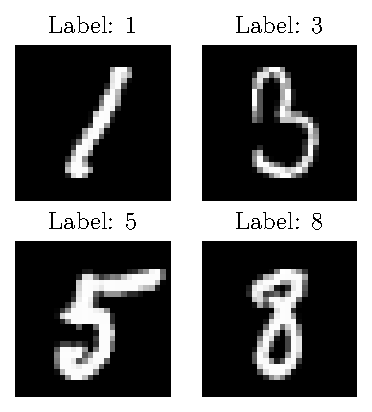
\includegraphics[width=.9\linewidth]{images/mnist_raw.pdf}
      \subcaption{Original.}
      \label{fig:mnist_dataset_original}
  \end{minipage}
  \begin{minipage}[b]{.4\linewidth}
      
\includegraphics[width=.9\linewidth]{images/mnist_binarized.pdf}
      \subcaption{Binarized.}
      \label{fig:mnist_dataset_binarized}
  \end{minipage}
  \caption{Samples from the original (\subref{fig:mnist_dataset_original}) and binarized (\subref{fig:mnist_dataset_binarized}) MNIST dataset. A LUT network can only do binary classification, so we have to binarize the labels as well. Numbers from 0-4 get the label 0 and numbers from 5-9 get the label 1.}
\label{fig:mnist_dataset}
\end{figure}

\subsubsection{Experiments from paper}
We construct a LUT network with five hidden layers of 1024 LUTs and one LUT in the output layer. Every LUT in the network takes eight bits as input. Construction of the network is performed with the training set with 60000 samples and after training we validate on the test set with 10000 samples. The code is written by ourselves in Python using the package Numpy \cite{harris2020array} for matrix operations. Similar to other machine learning packages, a LUT network object with provided arguments is first created and methods like \hl{\texttt{.train()}} and \hl{\texttt{.predict()}} allows the user to work with the LUT network at a high level. The code is available on GitHub \cite{lut_github}. We obtain a training accuracy of 0.89 and a test accuracy of 0.87 which are the exact results from \cite{chatterjee2018learning}. Note that the results are way above 0.5 meaning some learning had taken place. The way the LUT network is defined, every individual LUT already gives a prediction on the example passed to the network. That means we can compute the training (or testing) accuracy for every LUT in the network. Figure~\ref{fig:ex1_depth_performance} visualizes the training accuracy dependent on the layer. Each point represents the mean training accuracy over the respective layer and the total height of the error bars are two standard deviations. We can see that with increasing layer number, the accuracy goes up and the standard deviation goes down until it reaches zero at layer six because there is only one LUT in the last layer. Increasing performance with increasing depth reminds us of neural networks where adding more layers is a heuristic to increase performance.

\begin{figure}[!htb]
    \centering
    \includestandalone[]{standalone/lut/depth_performance}
    \caption{Training accuracy dependent on layer for an 8-LUT network with five hidden layers (six is the output layer with just one LUT) and 1024 LUTs per layer, trained on the binary MNIST dataset using our own code \cite{lut_github}. The points represent the mean over the respective layer with two standard deviations as total height of the error bars. Similar to neural networks, we can see that performance increases with increasing depth. These results are our own and are almost identical to \cite{chatterjee2018learning}.}
\label{fig:ex1_depth_performance}
\end{figure}
\FloatBarrier

The bit-size of the LUTs (denoted by $\delta$ in Algorithm~\ref{alg:LUT}) is a crucial hyperparameter. In another experiment, \cite{chatterjee2018learning} varies the bit-size from two to 16 with steps of two and observes the effect on training and test accuracy. The rest of the LUT network is the same as before. Figure~\ref{fig:ex1_k_acc} visualizes the results.

\begin{figure}[!htb]
    \centering
    \includestandalone[]{standalone/lut/k_acc_real}
    \caption{Training and testing accuracy on binary MNIST when the bit-size of a LUT newtwork with five hidden layers and 1024 LUT per layer is varied. Increasing the bit-size sufficiently drives the training error near perfection. As with machine learning models in general, the testing accuracy goes down with too much complexity, meaning we are overfitting. The underlying data to produce this plot is taken from \cite{chatterjee2018learning}.}
\label{fig:ex1_k_acc}
\end{figure}
\FloatBarrier

\subsubsection{Majority vote} \label{sec:majority_vote}
So far the final prediction came from a single LUT that takes input from the last hidden layer. Considering the same architecture as in the previous section, the last hidden layer has 1024 LUTs. If $k=8$ (i.e. the number of bits per LUT), then for the final prediction only eight of those 1024 LUTs will be used. Since every LUT is trained with the same label vector $y$, each one of these 1024 LUTs could theoretically be used for a final prediction too. That motivates us to try a \textit{wisdom of the crowd} technique, a majority vote mechanism that takes into account the predictions of all LUTs in the last hidden layer. The prediction that occurs most often will be chosen as the final one. The complete scheme can be seen in Algorithm~\ref{alg:majority_vote}. We conduct an experiment using a LUT network with five hidden layers and 1024 LUTs per layer, varying the bit-size from two to 10 with steps of one, predicting with and without majority vote each time. The result can be seen in Figure~\ref{fig:majority_vote}. We can see that for low bit-size, using a majority vote significantly boots the training and testing performance. For high bit-sizes a majority vote has less effect, but still enhances the testing performance a little. Interestingly, for $k=5$, all accuracies coincide. Since using a majority vote requires almost no extra computational effort and at worst the results stay the same, it seems to be a good technique for enhancing the network's performance.

\begin{algorithm}
  \caption{LUT network majority vote}
  \label{alg:majority_vote}
  \begin{algorithmic}
    \State Given binary vector $\bm{x}$ and \underline{trained} LUT network according to Algorithm~\ref{alg:LUT} with $l_L$ luts in the last hidden layer, perform a majority vote to predict
    \vspace{1em}
    \State Initialize empty list $\alpha = [\hspace{0.3em}]$
    \For{LUT $j = 1, \dots, j_L$ in the last hidden layer}
      \State Append prediction of LUT$_j$ on $\bm{x}$ to $\alpha$ (either 0 or 1)
      \If{$\sum\limits_{\alpha_j = 0} > \sum\limits_{\alpha_j = 1}$}
        \State Return 0
      \ElsIf{$\sum\limits_{\alpha_j = 0} < \sum\limits_{\alpha_j = 1}$}
        \State Return 1
      \Else
        \State Return random choice of $\{0, 1\}$
      \EndIf
    \EndFor
  \end{algorithmic}
\end{algorithm}

\begin{figure}[!htb]
    \centering
    \includestandalone[]{standalone/lut/majority_vote}
    \caption{Training and testing accuracies with or without using a majority vote mechanism for a LUT network with five hidden layers and 1024 LUTs per layer. The task is binary MNIST. For low bit-sizes, using a majority vote significantly enhances performance while the effect lessens with higher bit-sizes, but still enhances the testing accuracy a little. Interestingly, all accuracies coincide at $k=5$.}
\label{fig:majority_vote}
\end{figure}
\FloatBarrier

\subsubsection{Maximizing layer-wise mean accuracy while training} \label{sec:max_layer_acc}
As mentioned earlier, every LUT is trained with the same label vector $y$ and is able to give a prediction. With increasing hidden layer number, the LUTs get increasingly better. Figure~\ref{fig:acc_layer_normal} visualizes this using histograms. The underlying data is the training accuracy per LUT per hidden layer for an 8-LUT network with five hidden layers and 1024 LUTs per hidden layer applied on the binary MNIST dataset. The training accuracy of this LUT is 0.89 and the testing accuracy is 0.87, the same accuracies as in the first experiment. The $x$-axis represents the training accuracy. For each hidden layer, we divide the data in 10 equally-sized bins (in terms of the accuracy) from the minimum to maximum value. Then for each bin, we erect a bar, where the height represents the number of data points that fall into this bin. We can see that on average, the accuracy increases with hidden layer number and the spread of accuracies reduces dramatically. For hidden layer 1, the accuracies are worst and the spread is maximal. The worst LUTs on hidden layer 1 are only slightly better than chance. That motivates us to conduct an experiment in which we try to maximize the accuracy of the LUTs while training.

We conceptualize following algorithm: after training a layer, we discard the $n$ worst LUTs in that layer and establish $n$ new LUTs that are hopefully better. We said \enquote{hopefully} because the learning algorithm takes a random subset of columns of the previous layer, leaving it to chance if a new LUT will perform better in terms of accuracy. After obtaining those $n$ new LUTs, we score every LUT and again discard the $n$ worst LUTs until the mean accuracy does not change anymore. We thus set a \textit{patience}, i.e., a number of iterations after no change in mean accuracy we will move onto the next layer. The implementation is described in Algorithm~\ref{alg:max_layer_acc}. Starting another experiment, we again use an 8-LUT with 5 hidden layers and 1024 LUTs per layer and the binary MNIST dataset. The patience we set to 10 and $n=50$.

\begin{figure}[!htb]
    \centering
    \includestandalone[]{standalone/lut/acc_layer_normal}
    \caption{Histograms of training accuracies per hidden layer for an 8-LUT network with five hidden layers and 1024 LUTs per layer. The task is binary MNIST. For each hidden layer, the data is divided into 10 equally sized bins from minimum to maximum value. For each range, we erect a bar with the height equal to the number of data points that fall within that range. The overall accuracy of this network is 0.89 on the training set and 0.87 on the testing set.}
\label{fig:acc_layer_normal}
\end{figure}

\begin{algorithm}
  \caption{Maximizing layer-wise mean accuracy while training}
  \label{alg:max_layer_acc}
  \begin{algorithmic}
    \State Given binary dataset $\bm{X}$ with $N$ rows and binary label vector $y$, construct a LUT network with $L$ hidden layers where the training accuracy in each hidden layer is maximized. This algorithm modifies Algorithm~\ref{alg:LUT}.
    \vspace{1em}
    \State Choose additional hyperparameters:
    \Statein Number of LUTs $n$ to discard after each iteration
    \Statein Patience $p \in \mathds{N}$
    \For{$i = 1, \dots, L$}
      \State Train layer $L$ as in Algorithm~\ref{alg:LUT}
      \State $\text{no\_change} \in \mathds{N} \gets 0$
      \State $\text{best} \in \mathds{R} \gets 0$
      \While{$\text{no\_change} < p$}
        \State Discard $n$ worst performing LUTs on $(\bm{X}, y)$
        \State Append $n$ new LUTs trained on $(\bm{X}, y)$ to the current layer
        \State $\text{accs} \in \mathds{R}^N \gets $ accuracy of each LUT on $(\bm{X}, y)$
        \State $\text{curr} \in \mathds{R} \gets \text{mean}(\text{accs})$
        \If{$\text{curr} > \text{best}$}
          \State $\text{best} \gets \text{curr}$
          \State $\text{no\_change} \gets 0$
          \Else
            \State $\text{no\_change} \mathrel{+}= 1$
        \EndIf
      \EndWhile
    \EndFor
    \State The single LUT after the last hidden layer is created as usual
  \end{algorithmic}
\end{algorithm}

After running the aforementioned algorithm, we obtain a training accuracy of 0.90 and a testing accuracy of 0.88, slightly better than before. In Figure~\ref{fig:acc_layer_discard} we can see the accuracies per layer visualized using a histogram. Contrary to Figure~\ref{fig:acc_layer_normal}, the distributions are much more narrow now. After training we also tried prediction with a majority vote, but the accuracies did not change.

\begin{figure}[!htb]
    \centering
    \includestandalone[]{standalone/lut/acc_layer_discard}
    \caption{Histograms of training accuracies per hidden layer for an 8-LUT network with five hidden layers and 1024 LUTs per layer, applied on binary MNIST. For this network, the accuracy of each layer is optimized until it does not change anymore, yielding an overall accuracy of 0.90 on the training set and 0.88 on the testing set. The results of this network are slightly better (increase of 1\% training and testing accuracy) compared to the same network without optimization. Contrary to Figure~\ref{fig:acc_layer_normal}, the distributions are much narrower.}
\label{fig:acc_layer_discard}
\end{figure}

\noindent For a more complete picture, we vary the bit-size from two to 10 while trying to improve the layer-wise accuracy. There are again five hidden layers with 1024 LUTs per layer. The result can be seen in Figure~\ref{fig:increase_layer_acc}. We can see that pushing up the layer-wise accuracy does indeed help increase the overall accuracy, albeit only significantly for low bit-sizes. For high bit-sizes, the effect is smaller.


\begin{figure}[!htb]
    \centering
    \includestandalone[]{standalone/lut/increase_layer_acc}
    \caption{Training and test accuracies for $k$-LUT networks with five layers and 1024 LUTs per layer applied on binary MNIST. Solid lines and markers denote accuracies of networks where the layer-wise accuracies have been improved. For low bit-sizes, improving layer-wise accuracies has a significant effect on the overall performance, while for higher bit-sizes the effect is smaller.}
\label{fig:increase_layer_acc}
\end{figure}
\FloatBarrier

\subsubsection{Feature engineering} \label{sec:feature_engineering}
So far we have not done any more sophisticated feature engineering except making a binary version out of the original MNIST dataset. Since feature engineering is an integral part of machine learning in general, we try it too and see if there is any improvement of the model's performance. We conduct an experiment where we enhance the data by emphasizing the edges. Concretely, we create a copy of the original image and replace each pixel with black if the adjacent pixel has the same value and white if the adjacent pixel has a different value. We do this process both in $x$- and $y$-direction and add the results to the original image. Figure~\ref{fig:sobel_single} illustrates this technique for one example.

\begin{figure}[!htb]
    \centering
    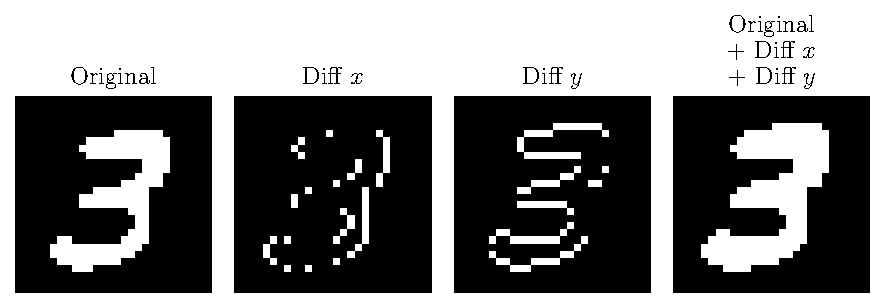
\includegraphics[width=.9\linewidth]{images/diff.pdf}
    \caption{Single example from the training data where we applied feature engineering. We create a copy of the original image and replace each pixel with black if the adjacent pixel has the same value and white if the adjacent pixel has a different value. We perform this process both in $x$- and $y$-direction and add the results to the original image. Looking at the feature engineered image on the right, the displayed number appears thicker.}
\label{fig:sobel_single}
\end{figure}
\FloatBarrier

\noindent Using the dataset enhanced with feature engineering, we train a LUT network with five hidden layers and 1024 LUTs per layer, varying the bit-size from two to 10. The result can be seen in Figure~\ref{fig:sobel_acc}. We can see that the accuracies are consistently higher for models that were trained on images where feature engineering had been applied. The technique described in this section was inspired by the Sobel operator \cite{sobelsobel} which calculates the gradients in an image in either $x$- or $y$-direction. Using this operator as feature engineering technique as opposed to our own produces similar results. We presented our own as main technique for the sake of an easier explanation and brevity.

\begin{figure}[!htb]
    \centering
    \includestandalone[]{standalone/lut/feature_engineering}
    \caption{Train and test accuracies for models trained on unmodified binary MNIST data and binary MNIST data where feature engineering had been applied. We can see that using feature engineering boosts the performance slightly.}
\label{fig:sobel_acc}
\end{figure}
\FloatBarrier

\subsubsection{Performance of various ML algorithms on binary MNIST} \label{sec:models}
As in \cite{chatterjee2018learning}, we train various Machine Learning algorithms on the binary MNIST dataset and compare their performance. The training and testing accuracies can be seen in Table~\ref{tab:ml_algos_on_bmnist}. Each LUT network has 5 hidden layers and 1024 luts per layer, except the \enquote{8-LUT network slim} which has 5 hidden layers and 256 luts per layer. For the reader wishing to refresh their knowledge about Convolutional Neural Networks, \cite{yamashita2018convolutional} provides a good overview. We implemented the CNN using the Python package PyTorch \cite{NEURIPS2019-9015}. The CNN has two convolutional layers with 64 and 32 filters and 2 fully connected layers with 256 and 128 neurons. After the convolutions, we perform max pooling and we use ReLU as activation function between the layers. The output has a sigmoid activation function. We use the Adam optimizer and go throgh the dataset only once, i.e., train for one epoch. For all other learning algorithms, we use the Python package scikit-learn \cite{scikit-learn}. Except the parameters that we explicitely state we use the default parameters from scikit-learn. We can see that a 12-LUT network beats Logistic Regression and Naïve Bayes. The best performing model is a Convolutional Neural Network. Our results are the same as in \cite{chatterjee2018learning}, take or leave 1\%.

Another interesting aspect to consider is how much disk space these models take up. In Table~\ref{tab:ml_algos_on_bmnist} the last column shows the size of all parameters for each model in Kilobytes, the derivation of which can be seen in Appendix~\ref{app:size}. Some models have no entry for the parameter size because they do not have any trainable parameters. Using the same architecture as \cite{chatterjee2018learning}, but varying the bit-size, we can see LUTs underperform compared to the CNN in both accuracy and size. A 10-LUT network might seem to have a good trade-off between accuracy and model size, but we need to consider that the convolutional neural network could be made much smaller by pruning \cite{molchanov2016pruning}. More impressive is the 8-LUT network with 5 hidden layers and 256 LUTs per layer. With 41 KB, it is 28 times smaller than the CNN and has almost the same testing accuracy as the 8-LUT network with 1024 luts per hidden layer.

\begin{table}[!htb]
    \begin{small}
        \begin{tabular}{llll}
        Algorithm & Training    & Testing    & Size of parameters \\
                  & accuracy    & accuracy   &                    \\ \hline
        Convolutional Neural Network & 0.99  & 0.99 & 1164 KB     \\
        5-Nearest Neighbors          & 0.99  & 0.97 & -           \\
        1-Nearest Neighbors          & 1.00  & 0.97 & -           \\
        Random Forests (10 trees)    & 1.00  & 0.96 & 3797 KB     \\
        \textbf{12-LUT network}      & 0.99  & 0.90 & 2622 KB     \\
        \textbf{10-LUT network}      & 0.94  & 0.88 & 655 KB      \\
        \textbf{8-LUT network}       & 0.89  & 0.87 & 164 KB      \\
        \textbf{8-LUT network slim}  & 0.88  & 0.87 & 41 KB       \\
        Logistic Regression          & 0.87  & 0.87 & 3 KB        \\
        Naïve Bayes                  & 0.77  & 0.77 & 16 KB       \\
        Random Guess                 & 0.50  & 0.50 & -  
        \end{tabular}
    \end{small}
    \caption{Performance of various ML algorithms on the binary MNIST dataset. How the sizes of the parameters were computed can be seen in Appendix~\ref{app:size}.}
\label{tab:ml_algos_on_bmnist}
\end{table}

\subsubsection{AdaBoost.M1} \label{sec:ada_boost}
In Section~\ref{sec:majority_vote}, as opposed to having one final LUT, we counted the number of output labels in the last hidden layer and took the label as final prediction whichever was occurring the most. We could view that as a \textit{wisdom of the crowd} technique. Now we try another ensembling method which is very well established in literature and practice, the AdaBoost.M1 algorithm \cite{adaboostm1}. It is a boosting method, meaning a classifier is built sequentially by training individual classifiers and adding them up. Every classifier is trained individually with the addition of weights that come from the previous iteration. Every sample in the training set is assigned a weight, with all weights equal to $1/N$ in the beginning, where $N$ is the number of samples. Given the current classifier and weights, for each iteration $n$ a number $\alpha_n$ is calculated. The final prediction for a sample $\bm{x}$ is $f(\bm{x}) = \text{sign}(\sum_{n=1}^{\mathcal{N}} \alpha_n f_n(\bm{x}))$. The full algorithm can be seen in Figure~\ref{alg:adaboostm1}.

\begin{algorithm}
  \caption{AdaBoost.M1 algorithm according to \cite{adaboostm1}} \label{alg:adaboostm1}
  \begin{algorithmic}
    \State Given dataset $(\bm{X}, \bm{y})$, where $\bm{X} = \bm{x}_1, \dots, \bm{x}_N$ and $\bm{y} = y_1, \dots, y_N$, $y_i \in \{-1, 1\}$ and model class, construct a classifier that is made up of $n$ individual classifiers $f_1, \dots, f_n$.
    \vspace{1em}
    \State Initialize weight vector $\bm{w} \in \mathds{R}^N$ with $w_{1, \dots, N} = 1/N$
    \vspace{0.5em}
    \For{$i = 1, \dots, n$}
    \State Train classifier $f_i$ on $(\bm{X},\bm{y})$ and weights $\bm{w}$
    \State $\text{err}_i \gets \big( \sum_k w_k \mathbb{1}(f_i(\bm{x}_k) \neq y_k) \big) / \sum_k w_k$
    \State $\alpha_i = \log((1 - \text{err}_i) / \text{err}_i)$
    \For{$k = 1, \dots, N$}
    \State $w_k \gets w_k \exp(\alpha_i \mathbb{1}(f_i(\bm{x}_k) \neq y_k))$
    \EndFor
    \EndFor
    \State Prediction on yet unseen $\bm{x}$: $\text{sign} \big( \sum_{i = 1}^n \alpha_i f_i(\bm{x}) \big)$
  \end{algorithmic}
\end{algorithm}

\begin{algorithm}
  \caption{LUT ensembling}\label{alg:lut_ensemble}
  \begin{algorithmic}
    \State Given dataset $(\bm{X}, \bm{y})$, where $\bm{X} = \bm{x}_1, \dots, \bm{x}_N$ and $\bm{y} = y_1, \dots, y_N$, $y_i \in \{-1, 1\}$ and model class, construct a classifier that is made up of $n$ individual classifiers $\text{LUT}_1, \dots, \text{LUT}_n$.
    \vspace{1em}
    \State Initialize weight vector $\bm{w} \in \mathds{R}^N$ with $w_{1, \dots, N} = 1/N$
    \vspace{0.5em}
    \For{$i = 1, \dots, n$}
    \State Train $\text{LUT}_i$ on $(\bm{X},\bm{y})$
    \State $\text{err}_i \gets \big( \sum_k w_k \mathbb{1}(\text{LUT}_i(\bm{x}_k) \neq y_k) \big) / \sum_k w_k$
    \State $\alpha_i = \log((1 - \text{err}_i) / \text{err}_i)$
    \For{$k = 1, \dots, N$}
    \State $w_k \gets w_k \exp(\alpha_i \mathbb{1}(\text{LUT}_i(\bm{x}_k) \neq y_k))$
    \EndFor
    \EndFor
    \State Prediction on yet unseen $\bm{x}$: $\text{sign} \big( \sum_{i = 1}^n \alpha_i \text{LUT}_i(\bm{x}) \big)$
  \end{algorithmic}
\end{algorithm}

\noindent As a first experiment, we apply the AdaBoost.M1 algorithm on a 2-LUT network with 5 layers and 1024 LUTs per layer. We vary the number of LUT networks from 2 to 1024. The motivation for choosing 2-LUT networks is computation time. Since we want to keep open the possibility for many LUT networks in the ensembled classifier, we have to restrict ourselves with the bit-size, otherwise it would take too long to train and predict. The results can be seen in Figure~\ref{fig:ada_2_LUT}. We can see that with an increasing number of LUT networks, we can indeed improve the accuracy. However, we can achieve the same results with a single LUT network if we set the bit-size to a sufficient level. Also train and inference time of a single LUT network with a higher bit-size is much faster than bunching together many small ones. Strictly speaking we do not fully follow the AdaBoost.M1 algorithm in this experiment. The algorithm requires for each training iteration to find an optimal classifier to the dataset \textbf{and} weights. If a weight is high, we should pay more attention to that sample in the next iteration and vice-versa if the weight is low. A LUT network during training considers all samples equal and there is no way of paying more attention to some and less to others.

\begin{figure}[!htb]
    \centering
    \includestandalone[]{standalone/lut/ada_2_LUT}
    \caption{Train and test accuracies for boosted models according to the AdaBoost.M1 algorithm where 2-LUT networks with 5 layers and 1024 LUTs per layer are the base classifiers. With increasing number of LUT networks, the accuracy improves. However, these results can also be achieved with a single LUT network where the bit-size is set sufficiently high. A single LUT network also has faster training and inference speed.}
\label{fig:ada_2_LUT}
\end{figure}
\FloatBarrier

\subsubsection{Random forests}
The basic idea of Random Forests is to reduce variance (i.e. improve model performance) by bunching many submodels that are (as best as possible) decorrelated. The submodels are decision trees. Decorrelation is achieved by training on only a subset of the whole training data for each individual decision tree and considering only a subset of all features during each split. We would like to apply a similar technique to LUT networks. As in the previous section, a classifier consists of many individual LUT networks. This time the final prediction will be made according to a majority vote. Considering only a subset of the whole training data for each individual LUT network we can achieve easily. As for the randomization during splits, LUT networks achieve this already by choosing a random subset of all columns. The final classifier thus consists of different LUT networks that have been trained on random subsets of the training data.

We conduct a new experiment where we try the described technique described above with an 8-LUT network with 5 layers and 1024 LUTs per layer as submodel. The number of submodels we set to 64. As opposed to AdaBoost.M1 from Section~\ref{sec:ada_boost}, the base classifiers here are more powerful. Generally, boosting methods bunch together many individual weak classifiers while Random Forests bunch together many individual strong classifiers. We obtain a training accuracy of 0.89 and testing accuracy of 0.87, no better than a single 8-LUT from our previous experiments.

\subsubsection{Combining different methods}
We combine different methods presented in previous sections, i.e. majority vote from Section~\ref{sec:majority_vote}, maximizing layer-wise mean accuracy while training from Section~\ref{sec:max_layer_acc} and feature engineering from Section~\ref{sec:feature_engineering}. We use an 8-LUT network with 5 layers and 1024 LUTs per layer. The number of LUTs to discard in each iteration we set to 50 with a patience of 5. We obtain a training accuracy of 0.93 and a testing accuracy of 0.92. For comparison, without optimization the training and testing accuracy are 0.89 and 0.87, respectively. Using only Sobel yields 0.91 and 0.89.
